\section{Wachstum}
\begin{multicols}{2}
\subsection{Langfristiger Wachstumstrend}
\includegraphics[width=\linewidth]{images/wachstum.png}
\columnbreak

\subsection{Quellen des Wachstums}
\includegraphics[width=\linewidth]{images/quellen.png}
\end{multicols}

\begin{multicols}{2}
\subsubsection{Exogene Faktoren}
\begin{itemize}
	\item Ausstattung mit Rohstoffen
	\item Klima
	\item Nähe zu Handelspartnern
	\item Sozialkapital
	\subitem politische Stabilität
	\subitem Ausgestaltung der politischen Rechte
	\subitem Vertrauen in Eigentums- und Vertragsrechte
	\subitem tiefe Korruption
\end{itemize}
\vfill\null
\columnbreak
\subsubsection{Mehr Arbeitsstunden}
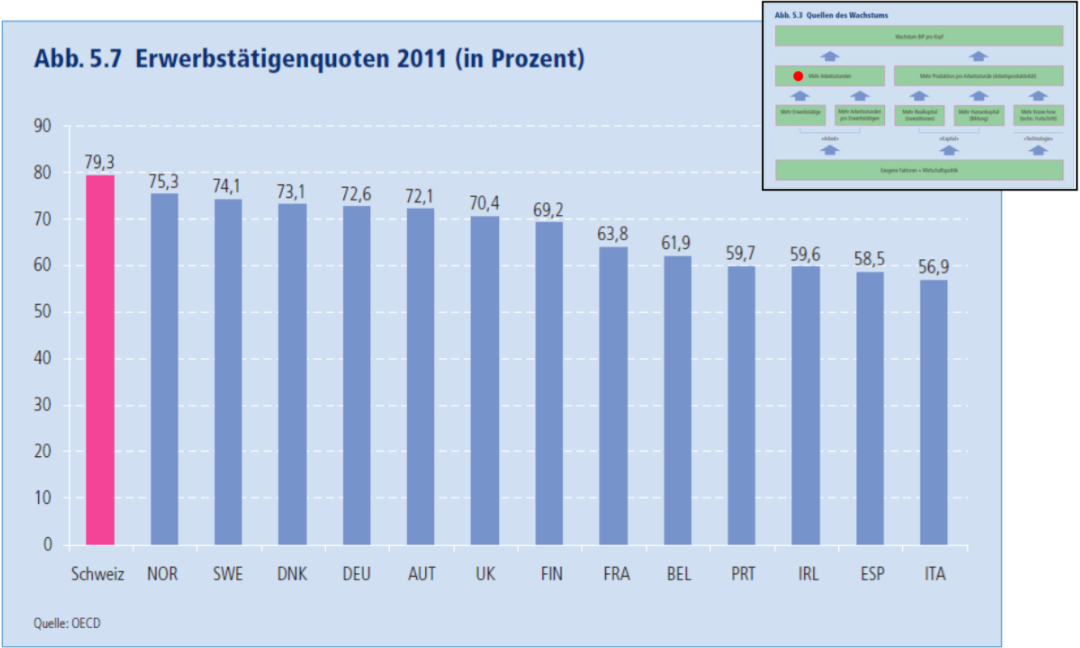
\includegraphics[width=\linewidth]{images/arbeitsstunden.png}
\end{multicols}

\begin{multicols}{2}
\subsubsection{Arbeitsproduktivität}
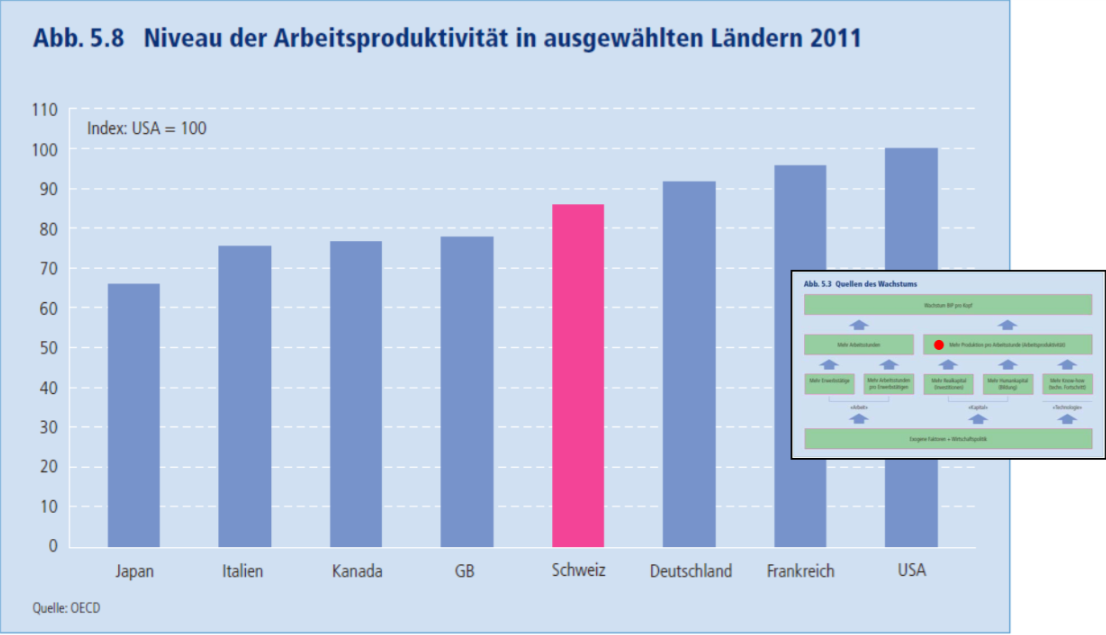
\includegraphics[width=\linewidth]{images/arbeitsproduktivitaet.png}
\textbf{Reales BIP / Anzahl Arbeitsstunden}
\columnbreak
\subsubsection{Staatsquote}
\begin{itemize}
	\item Staatsquote = (öffentlicher Konsum + öffentliche Investitionen) / nominales BIP
	\item Zunehmender staatsnaher Sektor (Erziehung, Gesundheit, Soziales und Energie) expandiert und wirkt als Bremse für das Wachstum
\end{itemize}
\end{multicols}

\subsubsection{Mehr Know-How (techn. Fortschritt = unendliche Ressource)}
Technologie ist das Wissen, auf welche Art Arbeit und Kapital kombiniert werden können, um Güter und Dienstleistungen zu produzieren. Techn. Fortschritt kann durch Forschung/Entwicklung (F\&E) erzielt werden, aber auch über den Lernprozess bei der Arbeit (Learning by Doing). Er ist der bei Weitem wirksamste Auslöser von Wachstum.\\
\textbf{Schutz des Geistigen Eigentums:} Wenn durch F\&E errungene Erträge sofort allen verfügbar gemacht würde, investierte niemand in F\&E, womit kein Wachstum erzielt würde. Deshalb gibt es Patentrechte:
\begin{itemize}
	\item Patentschutz (max. 20 Jahre)
	\item Designschutz (5 Jahre, verlängerbar auf max. 25 Jahre)
	\item Urheberrecht (70 Jahre nach Tod des Urhebers, 50 Jahre bei Software)
	\item Markenschutz (10 Jahre, beliebig verlängerbar)
\end{itemize}
Somit gibt es einen Anreiz in F\&E zu investieren, da man sich so einen (zeitlich begrenzten) Produktivitätsvorteil ggü. der Konkurrenz verschafft. Damit das gesamtwirtschaftliche Wachstum aber nicht leidet, sind diese Patentrechte zeitlich beschränkt, womit die gesamte Wirtschaft von Errungenschaften in der F\&E profitiert.

\begin{multicols}{2}
\subsubsection{Schweizer Wachstumsflaute}
\begin{itemize}
	\item Problem der Schweizer Hochpreisinsel (Abschottung Binnenmarkt)
	\item Höheres Wachstum der Schweizer Staatsquote
	\item Nicht schuld ist die höhere Immigration
\end{itemize}
\vfill\null
\columnbreak
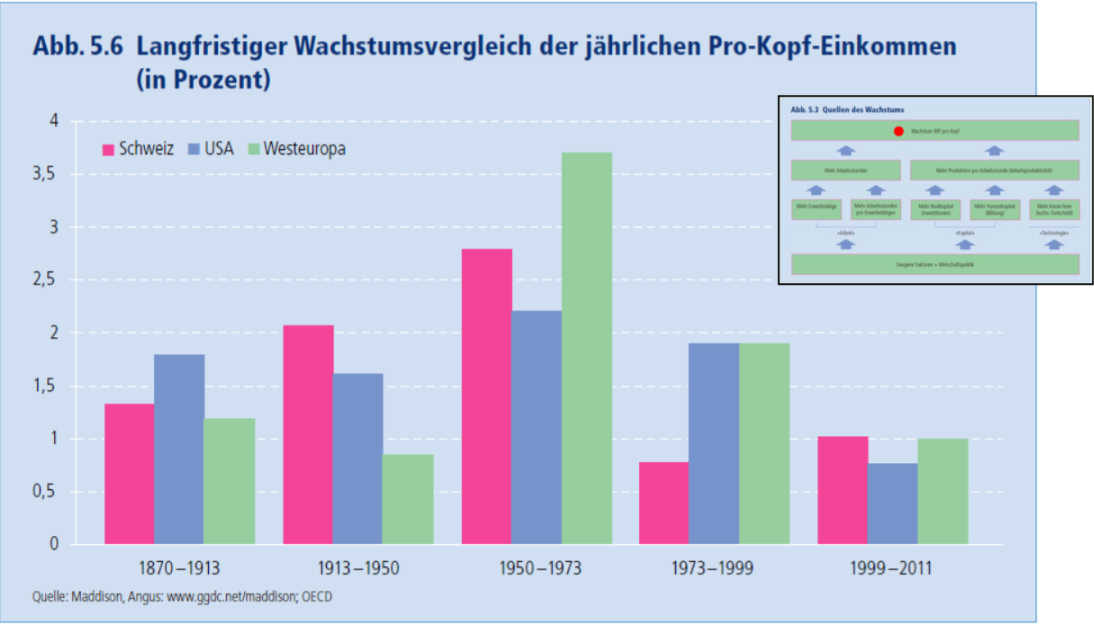
\includegraphics[width=\linewidth]{images/wachstumsvergleich.png}
\vfill\null
\end{multicols}

\subsubsection{Schweizer Wachstumspolitik I (2004-2007) (Schuldenbremse)}
\textbf{Ursachen der "Wachstumsflaute"}
\begin{itemize}
	\item Problem der Schweizer Hochpreisinsel
	\item Höheres Wachstum der Schweizer Staatsquote als andere OECD-Länder
\end{itemize}
\textbf{Zielsetzungen}
\begin{itemize}
	\item Erhöhung des Wettbewerbs auf dem Schweizer Binnenmarkt
	\begin{itemize}
		\item Reformen im Gesundheitswesen (noch nicht wirklich geschehen), Landwirtschaft (viele Subventionen), Strommarkt (immer noch Staatsmonopol)
	\end{itemize}
	\item Eindämmung des Wachstums der Staatsquote
	\begin{itemize}
		\item Einführung der Schuldenbremse (vom Volk durchgesetzt, soll abgeschwächt werden)
		\item Eliminierung des strukturellen Budgetdefizits
	\end{itemize}
	\item Effiziente Ausgestaltung staatlicher Tätigkeiten und Regulierungen
	\begin{itemize}
		\item Reform der Unternehmenssteuer, Mehrwertsteuer
		\item Administrative Entlastung der Unternehmen
	\end{itemize}
\end{itemize}

\subsubsection{Schweizer Wachstumspolitik II (2008-2011)}
\textbf{Wachstumspaket} mit 20 wirtschaftspolitischen Massnahmen:
\begin{itemize}
	\item Senkung des hohen Kostenniveaus (Hochpreisinsel)
	\item Attraktivitätssteigerung für Teilnahme am Erwerbsleben (RAV)
	\item Aufwertung des Unternehmensstandorts
\end{itemize}

\subsubsection{Schweizer Wachstumspolitik III (2012-2015) (Nachhaltigkeit)}
\textbf{Sieben Handlungsfelder der Wachstumspolitik} (13 Massnahmen):
\begin{itemize}
	\item die Behebung des Wettbewerbs im Binnenmarkt als Ziel der Wettbewerbspolitik
	\item die wirtschaftliche Öffnung nach aussen als Ziel der Aussenwirtschaftspolitik
	\item die Wahrung einer hohen Erwerbsbeteiligung als Ziel der Arbeitsmarktpolitik
	\item die Stärkung von Bildung, Forschung, Innovation als Ziel der Bildungs- und Arbeitsmarktpolitik
	\item die Gewährleistung gesunder öffentlicher Finanzen als Ziel der Finanzpolitik
	\item die Schaffung eines rechtlichen Umfeldes, das der unternehmerischen Initiative förderlich ist, als ein spezifischer Gegenstand der Rechtsetzung
	\item die Tragbarkeit der Umweltbeanspruchung gewährleisten als Ziel der Umweltpolitik
\end{itemize}

\subsubsection{Schweizer Wachstumspolitik IV (2016-2019) (Digitalisierung)}
Der Bundesrat hat am 21. Januar 2015 den Bericht $"$Grundlagen für die Neue Wachstumspolitik: Analyse der bisherigen und Ausblick auf die zukünftige Strategie$"$ verabschiedet. Er hält an der generellen Stossrichtung seiner Strategie fest und will weiterhin das Wirtschaftswachstum fördern, langfristig die Arbeitsplätze und den Wohlstand in unserem Land sichern.\\
Der Bundesrat zielt dabei vor allem auf die Steigerung der Arbeitsproduktivität sowie die Stärkung von Wettbewerbs- und Innovationsfähigkeit. Zudem sollen künftig die Widerstandsfähigkeit der Wirtschaft und die Milderung problematischer Nebenwirkungen des Wirtschaftswachstums stärker in die Strategie einfliessen.\\
Das Eidgenössische Departement für Wirtschaft, Bildung und Forschung WBF wird in Zusammenarbeit mit den betroffenen Departementen dazu konkrete Massnahmen erarbeiten und dem Bundesrat bis Ende 2015 vorlegen.

\clearpage
\pagebreak